\begin{tikzpicture}

%A matrix
\draw [fill=cyan, opacity=.2]  (-6.2,4) node (v1) {} rectangle (1.6,-0.2) node (v2) {};
\draw [thick] (v1) rectangle (1.6,3);
\draw [thick] (-6.2,3) rectangle (1.6,2);
\draw [thick] (-6.2,0.8) rectangle (v2);
\node at (-2.3,1.4) { \color{red}\Large  \bf  \vdots};
\node at (-2.3,3.5) {\color{red} \bf  \Large $\underline{a_1}$};
\node at (-2.3,2.5) { \color{red} \bf  \Large $\underline{a_2}$};
\node at (-2.3,0.3) {\color{red} \bf  \Large $\underline{a_m}$};
\node at (-2.3,-1.3) {\huge$ \underset{ \color{blue} ( m \ll n)}{A_{ m \times n} }$};

% X vector
\draw [ thick, fill=green] (4,5) rectangle (5,6);
\draw [thick] (5,5) rectangle (4,4);
\draw [thick, fill=green] (4,4) rectangle (5,3);
\draw [] (4,3) node (v4) {} rectangle (5,-0.1) node (v5) {};
\draw [thick] (4,-0.1) rectangle (5,-1.1);
\draw [thick, fill=green] (4,-1.1) rectangle (5,-2.1);
\node at (4.6,-3.2) {\huge $\underset{\tiny \color{blue} (K-sparse)}{x_{n \times 1 }} $};
\node at (4.5,1.6) {\Large \bf \vdots};
\node at (2.9,2.7) {\Huge $\times$};
\draw [thick] (v4) rectangle (5,2.1);
\draw [thick] (v5) rectangle (4,0.8);

% y

\draw [thick] (-10.35,4) node (v3) {} rectangle (-9.35,3);
\draw [thick] (-10.35,3) rectangle (-9.35,2);
\draw [thick] (-10.35,2) rectangle (-9.35,0.9);
\draw [thick] (-10.35,0.9) rectangle (-9.35,-0.1);
\draw[fill=red, opacity=0.2]  (v3) rectangle (-9.35,-0.1);


\node at (-9.85,1.5) {\bf \vdots};

\node at (-7.85,2) {\Huge = };
\node at (-9.85,-1.2) {\huge $ \underset{ \color{blue} (sketch \ of \ x) }{y_{m \times 1}}$};

\end{tikzpicture}